\section{Versuchsaufbau/-durchführung}

\subsection{Versuchsaufbau}
Im Versuch US $1$ wird ein Ultraschallechoskop, eine Ultraschallsonde und ein Rechner %sonde
zum Verarbeiten der Daten verwendet.
Die Messdaten werden vom Computer mittels eines A-Scan angezeigt.
Als Probe werden aus Acryl gefertigte Zylinder und Quader verwendet.
Zusätzlich wird auch ein Augenmodell (vgl. \ref{fig: auge}) untersucht. %modell
Die Messungen werden im Impuls-Betrieb des Echoskop durchgeführt. Als Messverfahren werden
das Impuls-Echo-Verfahren und das Durchschallungs-Verfahren benutzt. Das Echoskop kann mittels
eines Kippschalters auf eines der beiden Verfahren eingestellt werden.
Die verwendete Sonde arbeitet in einem Bereich von $0-35\,\map{dB}$ und mit einer
Frequenz von $\SI{2}{\mega\hertz}$.
Wie in der Theorie angesprochen besitzt Luft einen hohen Absorptionskoeffizient, deshalb wird %angesprochen, Absorptionskoeffizient
auf den Proben entweder \emph{bidestilliertes Wasser} oder eine spezielle \emph{Kontaktcreme} %spezielle nicht kursiv
als Kontaktmedium aufgetragen.
Die Höhe von jedem Zylinder und Quader wird zu  Beginn des Versuches vermessen. %absätze
\subsection{Bestimmung der Dämpfung und der Schallgeschwindigkeit mit dem Impuls-Echo-Verfahren}
Der zu untersuchende Zylinder wird auf ein Papiertuch gestellt und anschließend
mit bidestilliertem Wasser benetzt. Die Sonde, im Impuls-Echo-Modus, wird auf dem
Zylinder platziert. An dem Computer sind nun zwei Peaks zu erkennen. Der erste Peak
entsteht beim Eintreten des Schalles in die Probe. Hingegen wird der zweite Peak
durch die reflektierte Welle erzeugt. Die Amplitude und die Laufzeit der Peaks
werden aus dem vom Computer erzeugten A-Scan abgelesen und notiert.
Insgesamt werden $7$ Zylinder untersucht.

\subsection{Bestimmung der Schallgeschwindigkeit mit dem Durschallungs-Verfahren}

Die Arcylzylinder werden auf eine Halterung gelegt, von beiden Seiten wird
mit der Kontaktcreme eine Sonde gekoppelt. Das Echoskop befindet sich im
Durchschallungsmodus. Aus dem erzeugten A-Scan kann die Durchlaufzeit der
Schallwelle bestimmt und aufgeschrieben werden. Die Messung wird für alle unterschiedlich
hohen Zylinder wiederholt.

\subsection{Untersuchung am Spektrum und Ceptstrum}

Für diesen Versuchsteil werden zwei Acrylscheiben und ein Zylinder (Höhe $\approx \SI{40}{\milli\meter}$)
gestapelt und dabei mit bidestilliertem Wasser gekoppelt, ebenso die Sonde.
Auf dem A-Scan sollte nun ein Mehrfachecho (drei Peaks) erkennbar sein.
Neben dem eigentlichen A-Scan zeigt der Computer auch das Spektrum und das Cepstrum des
eingegangenen Signals auf. %signals
Das Ceptstrum gibt die logarithmierte inverse Fouriertransformation an.
Mit Hilfe des Spektrums und des Cepstrums sollen die Laufzeiten der reflektierten Wellen
bestimmt werden.

\subsection{Untersuchung eines Augenmodells}

Der schematische Aufbau des benutzten Auges ist in Abbildung \ref{fig: auge} dargestellt.
\begin{figure}[h]
  \centering
  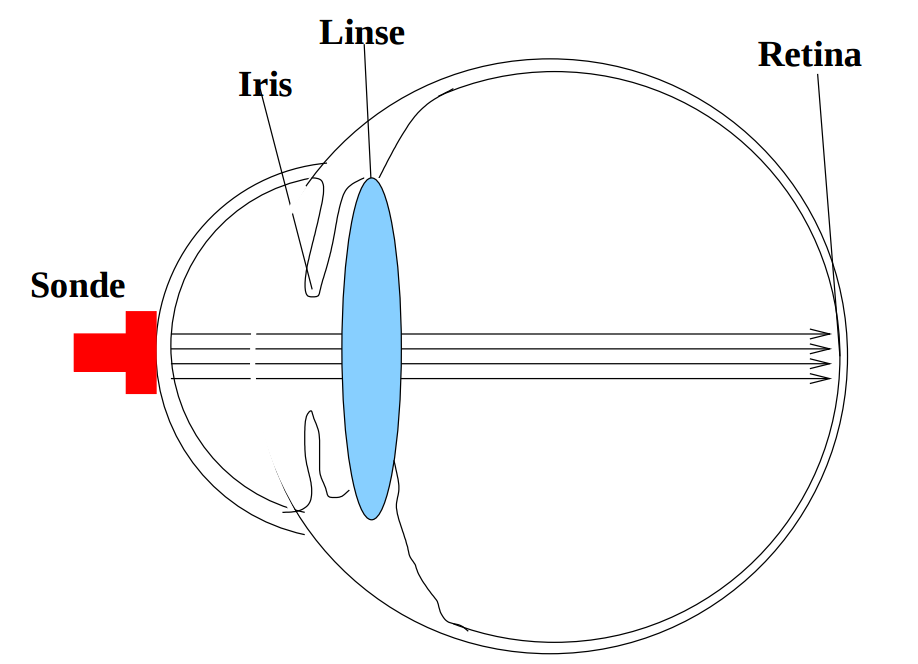
\includegraphics[width=0.4\textwidth]{pics/auge.png}
  \caption{Schematischer Aufbau des Auges \cite{anleitungus1}.}
  \label{fig: auge}
\end{figure}
Mit der Ultraschallechographie ist es möglich, den Abstand der Hornhaut, Iris, Linseneingang, Linsenausgang
und der Retina (reflektiert den Schall) zur Augenöffnung zu bestimmen.
Hierzu wird das Echo-Impuls Verfahren der Sonde und Kontaktcreme verwendet.
Die Sonde wird so lange mit leichtem Druck das Augenmodel gefahren, bis auf dem
A-Scan fünf Ausschläge erkennbar sind.
